\section{Matrix completion}

The goal of matrix completion is to fill in the missing entries of a sparse matrix $\mat{A}$. For
example, Netflix might want to use matrix completion to predict which users will give which ratings
to which movies, given the ratings given by all users of Netflix. However, not all users have rated
all movies, thus the matrix is sparse and must thus be filled in. Netflix can use this prediction
to decide which movies they should recommend to their users.

If we assume that all entries are independent, then no information is carried by one entry about
another. Because of this, we cannot reconstruct the matrix. Thus, we need to make an assumption
about the dependency within the matrix. A minimal assumption that we can make is that entries
within the same row or the same column are not independent, \ie, \[
    a_{ij} \ind \{ a_{kl} \mid k \neq i \land l \neq j \} \mid \{ a_{il} \mid l \neq j \} \cup \{ a_{kj} \mid k \neq i \}.
\]
This states that $a_{ij}$ is independent from all entries not on the same row or column, given that
we know all entries on the same row or column. However, in reality, we do not have all values on
the row and column for all entries. Thus, effectively, we have an indirect coupling between all
entries, since $a_{kl}$ influences $a_{kj}$ and $a_{il}$ (if they are unknown), which influence
$a_{ij}$.

Formally, we have a rating matrix $\mat{A} \in \R^{n \times m}$ and an observation matrix
$\mat{\Omega} \in \{ 0,1 \}^{n\times m}$, where $\omega_{ij}=1$ means that $a_{ij}$ is observed.
The goal is to predict all values $a_{kl}$, where $\omega_{kl}=0$.

A possible issue with the values is that some users might generally give higher ratings than
others.\sidenote{While it makes more sense intuitively that we should normalize ratings per user,
    it has been shown to be more effective to normalize items.} Thus, we want to account for this by
variance normalization. We can do this per row (user) or per column (item), where the two means can
be computed by \[
    \mu_i^{\mathrm{row}} = \frac{\sum_{j=1}^{m} \omega_{ij} a_{ij}}{\max \{ 1, \sum_{j=1}^{m} \omega_{ij} \}}, \quad \mu_j^{\mathrm{col}} = \frac{\sum_{i=1}^{n} \omega_{ij} a_{ij}}{\max \{ 1, \sum_{i=1}^{n} \omega_{ij} \}}.
\]
We then normalize by \[
    Z = \frac{X - \mu}{\sigma}.
\]

To approximate $\mat{A} \in \R^{n \times m}$, we will make the assumption that $\mat{A}$ is a
rank-$k$ matrix and approximate it by the product of two matrices $\mat{U} \in \R^{n \times k}$ and
$\mat{V} \in \R^{m \times k}$, \[
    \mat{A} \approx \mat{U} \transpose{\mat{V}}.
\]
Then, we get the following loss function that we wish to minimize, \[
    \mat{U}, \mat{V} \in \argmin_{\mat{U}, \mat{V}} \ell(\mat{U}, \mat{V}) \doteq \frac{1}{2} \lft\| \Pi_{\mat{\Omega}} \lft( \mat{A} - \mat{U}\transpose{\mat{V}} \rgt) \rgt\|_F^2,
\]
where $\Pi_{\mat{\Omega}}(\mat{M}) = \mat{M} \odot \mat{\Omega}$ and $\| \cdot \|_F$ is the
Frobenius norm, \[
    \| \mat{M} \|_F^2 = \sum_{i=1}^{n} \sum_{j=1}^{m} m_{ij}.
\]
This can be viewed as $\vec{u}_i \in \R^k$ representing each user and $\vec{v}_j \in \R^k$
representing each movie. Their dot product is the predicted value of $\vec{a}_{ij}$. Furthermore,
we have that $\mat{U}$ and $\mat{V}$ are fully determined by the observed values, but can be used
to extrapolate to a full matrix, achieving our objective.

\subsection{Fully observed case}

In this section, we consider the fully observed case, where $\omega_{ij}=1$ for all $i \in [n],
    j\in [m]$. Thus, we optimize \wrt the following loss function, \[
    \ell(\mat{U}, \mat{V}) = \frac{1}{2} \lft\| \mat{A} - \mat{U}\transpose{\mat{V}} \rgt\|_F^2,
\]

\begin{marginfigure}
    \centering
    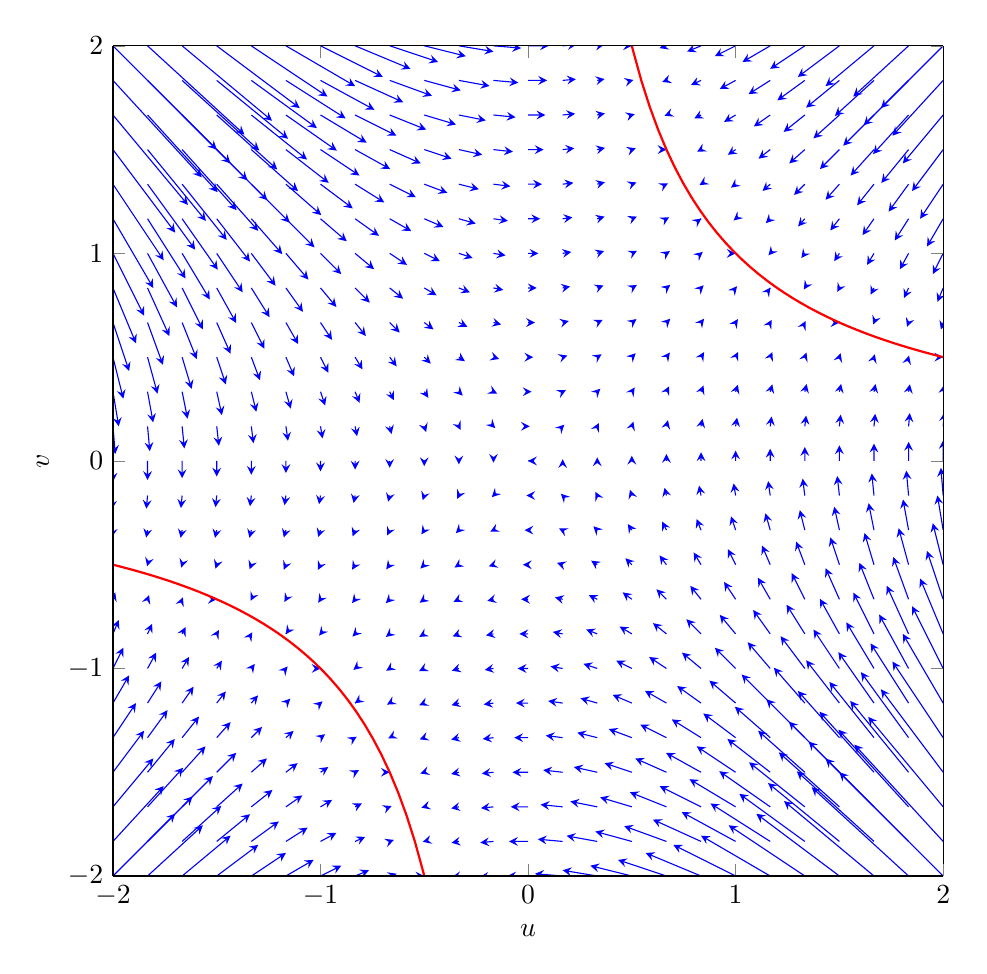
\begin{tikzpicture}
        \begin{axis}[
                xmin=-2, xmax=2,
                ymin=-2, ymax=2,
                axis equal image,
                xtick distance=1,
                ytick distance=1,
                view={0}{90},
                width=\textwidth,
                height=\textwidth,
                xlabel=$u$,
                ylabel=$v$
            ]
            \addplot3[
                blue,
                quiver={
                        u={-(x*y-1)*y},
                        v={-(x*y-1)*x},
                        scale arrows=0.05,
                    },
                -stealth,
                domain=-2:2,
                domain y=-2:2,
            ] {0};
            \addplot [red, thick, samples=100, domain=-2:2, restrict y to domain=-10:10] {1/x};
        \end{axis}
    \end{tikzpicture}
    \caption{Negative gradient field for $a=1$ in the scalar case with minima indicated by red. As can be seen, $[0,0]$ is a 2-way saddle point and any vector $[-z,z]$ for $z\in\R$ moves toward it. We can start at any other point and use gradient-based optimization to converge to the minimum.}
    \label{fig:grad-field}
\end{marginfigure}

\paragraph{Scalar case.}

To observe the properties of the gradients, we will first consider the 1-dimensional case, where $a
    \approx uv$, with $u,v\in\R$. We have the following loss function, \[
    \ell(u,v) = \frac{1}{2} (a - uv)^2.
\]
We thus have the following gradients,
\begin{align*}
    \delta              & = uv - a    \\
    \pdv*{\ell(u,v)}{u} & = \delta v  \\
    \pdv*{\ell(u,v)}{v} & = \delta u,
\end{align*}
which induces the negative gradient field shown in \Cref{fig:grad-field}. Furthermore, we have the following Hessian, \[
    \hess{\ell(u,v)}{} = \begin{bmatrix}
        v^2     & 2uv - a \\
        2uv - a & u^2
    \end{bmatrix}.
\]

\begin{lemma}[Second-order characterization of convexity]
    If $f: \mathcal{X} \to \R$ is twice differentiable, then $f$ is convex if and only if \[
        \hess{f(\vec{x})}{} \succeq \mat{0}, \quad \forall \vec{x} \in \mathrm{Int}(\mathcal{X}).
    \]
\end{lemma}

At the origin, we have the following Hessian, \[
    \hess{\ell(0,0)}{} = \begin{bmatrix}
        0  & -a \\
        -a & 0
    \end{bmatrix}.
\]
Thus, in the scalar case, the objective function is non-convex for $a \neq 0$. The same result can
be generalized to any $n,m \geq 1$. This means that we do not have any general convergence
guarantees using gradient-based methods. However, we can make guarantees if we study the gradient
flow of the loss function with ordinary differential equations (ODE).

Consider a balanced initialization $u_0 = v_0$. We see that $u$ and $v$ will evolve identically,
because their partial derivatives are equal in this case. We have the following update rule, \[
    u_t = u_{t-1} - \eta \pdv*{\ell(u,v)}{u} = u_{t-1} - \eta v(uv - a),
\]
where $\eta$ is an arbitrarily small stepsize. We then have the following ODE, \[
    \odv{u}{t} = \frac{u_t - u_{t-1}}{\eta} = -v(uv - a).
\]
Consider $x = uv$, then we have the following ODE, \[
    \odv{x}{t} = -2uv(uv-a) = -2x(x-a).
\]
Solving this ODE yields the following solution for $x(t)$, \[
    x(t) = a + \frac{ac - a^2}{ce^{2at} + a - c} \overset{t\to\infty}{=} a.
\]
In conclusion, starting from a balanced initialization, gradient descent with a small enough $\eta$
will converge $uv$ to $a$.

\paragraph{Rank-1 model.}

Now consider the fully observed rank-1 model,
\begin{align*}
    \ell(\vec{u}, \vec{v}) & = \frac{1}{2} \| \mat{A} - \vec{u}\transpose{\vec{v}} \|_F^2, \quad \mat{A} \in \R^{n \times m}, \vec{u} \in \R^n, \vec{v} \in \R^m                                                                                                                           \\
    \intertext{Rewriting,}
                           & = \frac{1}{2} \tr{\transpose{\lft( \mat{A} - \vec{u}\transpose{\vec{v}} \rgt)} \lft( \mat{A} - \vec{u}\transpose{\vec{v}} \rgt)} \margintag{Identity: $\| \mat{M} \|_F^2 = \tr{\transpose{\mat{M}}\mat{M}}$.}                                                 \\
                           & = \frac{1}{2} \tr{\transpose{\mat{A}}\mat{A} - \vec{v}\transpose{\vec{u}} \mat{A} - \transpose{\mat{A}}\vec{u}\vec{v} + \vec{v}\transpose{\vec{u}}\vec{u}\transpose{\vec{v}}}                                                                                 \\
                           & = \frac{1}{2} \lft( \tr{\transpose{\mat{A}}\mat{A}} - \tr{\vec{v}\transpose{\vec{u}} \mat{A}} - \tr{\transpose{\mat{A}}\vec{u} \vec{v}} + \tr{\vec{v}\transpose{\vec{u}}\vec{u}\transpose{\vec{v}}} \rgt) \margintag{Linearity of trace.}                     \\
                           & = \frac{1}{2} \lft( \tr{\transpose{\mat{A}}\mat{A}} - \tr{\transpose{\vec{u}} \mat{A} \vec{v}} - \tr{\transpose{\vec{v}} \transpose{\mat{A}} \vec{u}} + \tr{\transpose{\vec{v}}\vec{v}\transpose{\vec{u}}\vec{u}} \rgt) \margintag{Cyclic property of trace.} \\
                           & = \frac{1}{2} \tr{\transpose{\mat{A}}\mat{A}} + \frac{1}{2} \| \vec{u} \|^2 \| \vec{v} \|^2 - \transpose{\vec{u}} \mat{A} \vec{v}.
\end{align*}
The first term is a constant, thus we have the following effective loss function, \[
    \ell(\vec{u}, \vec{v}) = \frac{1}{2} \| \vec{u} \|^2 \| \vec{v} \|^2 - \transpose{\vec{u}} \mat{A} \vec{v}.
\]
We notice that the direction of $\vec{u}$ and $\vec{v}$ is fully decided by the second term. Thus,
if we first solve for that, we can then easily solve for the norm of the two vectors by also
considering the first term.

Specifically, let $\vec{u} = c_1 \tilde{\vec{u}}$ and $\vec{v} = c_2 \tilde{\vec{v}}$, such that
$\| \tilde{\vec{u}} \| = \| \tilde{\vec{v}} \| = 1$, and $c = c_1 \cdot c_2$. Then, we have the
following loss function with an additional parameter $c$, \[
    \ell(\tilde{\vec{u}}, \tilde{\vec{v}}, c) = \frac{1}{2} c^2 - c \transpose{\tilde{\vec{u}}} \mat{A} \tilde{\vec{v}}.
\]
Thus, we first maximize $\transpose{\tilde{\vec{u}}} \mat{A} \tilde{\vec{v}}$ under the constraint
that $\vec{u}$ and $\vec{v}$ are unit vectors, and then decide which $c$ minimizes the loss
function. Thus, first we have the following problem \[
    \vec{u}, \vec{v} \in \argmax_{\| \vec{u} \| = \| \vec{v} \| = 1} \transpose{\vec{u}} \mat{A} \vec{v}.
\]
We can solve this problem with its constraints by using Lagrangian multipliers, \[
    \mathcal{L} = \transpose{\vec{u}} \mat{A} \vec{v} - \alpha (\| \vec{u} \|^2 - 1) - \beta (\| \vec{v} \|^2 - 1).
\]
Using the first-order optimality condition, we get the following solutions,
\begin{align*}
    \grad{\mathcal{L}}{\vec{u}} = \mat{A} \vec{v} - 2 \alpha \vec{u} \overset{!}{=} 0 \; \implies \; \vec{u}            & = \frac{\mat{A} \vec{v}}{\| \mat{A} \vec{v} \|}                          \\
    \grad{\mathcal{L}}{\vec{v}} = \transpose{\mat{A}} \vec{u} - 2 \beta \vec{v} \overset{!}{=} 0 \; \implies \; \vec{v} & = \frac{\transpose{\mat{A}} \vec{u}}{\| \transpose{\mat{A}} \vec{u} \|}.
\end{align*}
Thus, the solutions must satisfy \[
    \vec{u} \propto \lft( \mat{A}\transpose{\mat{A}} \rgt) \vec{u}, \quad \vec{v} \propto \lft( \transpose{\mat{A}} \mat{A} \rgt) \vec{v}.
\]
As a result, we know that $\vec{u}$ should be proportional to an eigenvector of $\mat{A}
    \transpose{\mat{A}}$ and $\vec{v}$ should be proportional to an eigenvector of $\transpose{\mat{A}}
    \mat{A}$. Using this fact, we can rewrite the objective as
\begin{align*}
    \transpose{\vec{u}} \mat{A} \vec{v} & = \frac{\transpose{\vec{u}} \mat{A}  \transpose{\mat{A}} \vec{u}}{\| \transpose{\mat{A}} \vec{u} \|}                                                                                         \\
                                        & = \frac{\transpose{\vec{u}} \lambda \vec{u}}{\sqrt{\transpose{\vec{u}} \mat{A} \transpose{\mat{A}} \vec{u}}}                                                                                 \\
                                        & = \frac{\transpose{\vec{u}} \lambda \vec{u}}{\sqrt{\transpose{\vec{u}} \lambda \vec{u}}} \margintag{$\lambda$ is the eigenvalue of $\mat{A}\transpose{\mat{A}}$ corresponding to $\vec{u}$.} \\
                                        & = \frac{\lambda \| \vec{u} \|^2}{\sqrt{\lambda} \| \vec{u} \|}                                                                                                                               \\
                                        & = \sqrt{\lambda}. \margintag{$\vec{u}$ is a unit vector.}
\end{align*}
In order to maximize this term, we must thus select $\vec{u}$ and $\vec{v}$ to be the principal
eigenvectors of their respective matrices. Furthermore, $\ell(\tilde{\vec{u}}, \tilde{\vec{v}}, c)$
with this selection of $\tilde{\vec{u}}$ and $\tilde{\vec{v}}$ is minimized by selecting $c =
    \sqrt{\lambda_1}$, where $\lambda_1$ is the principal eigenvalue of $\mat{A}\transpose{\mat{A}}$
and $\transpose{\mat{A}} \mat{A}$.

In conclusion, the loss for a rank-1 model is minimized by selecting \[
    \mat{A} = \sqrt{\lambda_1} \vec{u} \transpose{\vec{v}},
\]
where $\vec{u}$ and $\vec{v}$ are the principal eigenvectors of $\mat{A} \transpose{\mat{A}}$ and
$\transpose{\mat{A}} \mat{A}$, and $\lambda_1$ is the principal eigenvalue. We can compute these
vectors by the power iteration algorithm.

\paragraph{Rank-$k$ model.}

We can generalize the previous result by making use of the singular value decomposition.

\begin{theorem}[SVD theorem]
    For each matrix $\mat{A} \in \R^{n \times m}$, there exists a diagonal matrix $\mat{\Sigma} \in
        \R^{n \times m}$ with ordered entries $\sigma_i \geq \sigma_{i+1} \geq 0, \forall i \in
        \min\{ n,m \}$ and orthogonal matrices $\mat{U} \in \R^{n \times n}, \mat{V} \in \R^{m\times
            m}$ such that $\mat{A}$ can be expressed as \[
        \mat{A} = \mat{U} \mat{\Sigma} \transpose{\mat{V}}.
    \]
\end{theorem}

\begin{lemma}
    \label{lem:svd-frob}
    Let the SVD of $\mat{A} \in \R^{n \times m}$ be given by $\mat{A} = \mat{U} \mat{\Sigma} \transpose{\mat{V}}$, then \[
        \| \mat{A} \|_F^2 = \sum_{i=1}^{\min\{n,m\}} \sigma_i^2.
    \]
\end{lemma}

\begin{proof}
    This can be shown by the properties of the trace operator,
    \begin{align*}
        \| \mat{A} \|_F^2 & = \tr{\transpose{\mat{A}} \mat{A}} = \tr{\mat{V} \transpose{\mat{\Sigma}} \transpose{\mat{U}} \mat{U} \mat{\Sigma} \transpose{\mat{V}}} = \tr{\mat{V} \transpose{\mat{\Sigma}} \mat{\Sigma} \transpose{\mat{V}}} \\
                          & = \tr{\transpose{\mat{V}} \mat{V} \transpose{\mat{\Sigma}} \mat{\Sigma}} = \tr{\transpose{\mat{\Sigma}} \mat{\Sigma}} = \sum_{i=1}^{\min \{ n,m \}} \sigma_i^2.
    \end{align*}
\end{proof}

\begin{lemma}
    Let the SVD of $\mat{A} \in \R^{n \times m}$ be given by $\mat{A} = \mat{U} \mat{\Sigma} \transpose{\mat{V}}$, then \[
        \| \mat{A} \|_2 \doteq \sup_{\| \vec{x} \| = 1} \| \mat{A} \vec{x} \| = \sigma_1. \margintag{Spectral norm.}
    \]
\end{lemma}

\begin{proof}
    We use the fact that orthogonal matrices preserve the Euclidean norm,
    \begin{align*}
        \sup_{\| \vec{x} \| = 1} \| \mat{A} \vec{x} \| & = \sup_{\| \vec{x} \| = 1} \| \mat{U} \mat{\Sigma} \transpose{\mat{V}} \vec{x} \| = \sup_{\| \vec{x} \| = 1} \| \mat{\Sigma} \transpose{\mat{V}} \vec{x} \| \\
                                                       & = \sup_{\| \vec{z} \| = 1} \| \mat{\Sigma} \vec{z} \| = \| \mat{\Sigma} \|_2 = \sigma_1.
    \end{align*}
\end{proof}

The Eckart-Young theorem is widely used for linear matrix approximation. It states that if we prune
the singular values below $\sigma_k$ in the SVD representation, we get an optimal rank-$k$
approximation of a matrix.

\begin{theorem}[Eckart-Young theorem]
    Let the SVD of $\mat{A} \in \R^{n \times m}$ be given by $\mat{A} = \mat{U} \mat{\Sigma}
        \transpose{\mat{V}}$. Then, for all $1 \leq k \leq \min\{n, m\}$, we have \[
        \mat{A}_k \doteq \mat{U} \mathrm{diag}([\sigma_1, \ldots, \sigma_k]) \transpose{\mat{V}} \in \argmin_{\mathrm{rank}(\mat{B}) \leq k} \| \mat{A} - \mat{B} \|_F.
    \]
\end{theorem}

From this, we can easily find a rank-$k$ approximation by \[
    \mat{A} \approx \sum_{i=1}^{k} \sigma_i \vec{u}_i \transpose{\vec{v}}.
\]
Furthermore, we can directly compute the squared error of low rank approximations as \[
    \| \mat{A} - \mat{A}_k \|_F^2 = \sum_{i=k+1}^{\mathrm{rank}(\mat{A})} \sigma_i^2.
\]
The SVD is computable in $\bigo{\min \{ nm^2, mn^2 \}}$, which is fast for a non-convex problem.
However, we cannot use this technique in the case of incomplete observations.

\subsection{Incompletely observed case}

In practice, the matrix $\mat{A}$ is often incompletely observed, meaning that we can only compute
the loss function \wrt the observed entries. This task is called ``Matrix completion'', and we
cannot use SVD in this case. Even worse, this problem is NP-hard, thus we have to resort to
approximation algorithms.

\paragraph{Alternating least squares.}

As we saw, we parametrize the approximation of $\mat{A}$ as a factorization of two matrices
$\mat{U} \in \R^{n \times k}$ and $\mat{V} \in \R^{m \times k}$, \[
    \mat{A} \approx \mat{U} \transpose{\mat{V}}.
\]
Since we cannot solve the problem exactly, we want to add regularization to the loss function to
increase numerical stability of the solution (this will also be very important later), \[
    \ell(\mat{U}, \mat{V}) = \frac{1}{2} \lft\| \Pi_{\mat{\Omega}}\lft( \mat{A} - \mat{U} \transpose{\mat{V}} \rgt) \rgt\|^2_F + \frac{\lambda}{2} \lft( \| \mat{U} \|_F^2 + \| \mat{V} \|_F^2 \rgt), \quad \lambda > 0.
\]
If we fully expand the norms, we will find that this objective is a 4-th degree polynomial in the
parameters (entries of $\mat{U}$ and $\mat{V}$) with the following monomials,
\begin{align*}
    \omega_{ij} u_{ir} v_{jr} u_{is} v_{js}, & \quad 1 \leq r, s \leq k \\
    \omega_{ij} u_{ir} v_{jr},               & \quad 1 \leq r \leq k    \\
    u_{ir}^2,                                & \quad 1 \leq r \leq k    \\
    v_{jr}^2,                                & \quad 1 \leq r \leq k.
\end{align*}
Importantly, every 4-th order term involves exactly one row index $i$ of $\mat{U}$ and one row index
$j$ of $\mat{V}$. In other words, the objective \wrt $\vec{u}_i$ depends further only on $\mat{V}$ and not any
other row of $\mat{U}$.\sidenote{The parameter dependencies form a bipartite graph between the rows of
    $\mat{U}$ and $\mat{V}$.} Using this information, we can separate out part of the objective
function depending on a row $\vec{v}_j$, where we treat $\mat{U}$ as fixed,
\begin{align*}
    \ell_{\mat{U}}(\vec{v}_j) & = \frac{1}{2} \lft\| \Pi_{\mat{\Omega}}\lft( \mat{A} - \mat{U} \transpose{\mat{V}} \rgt) \rgt\|_F^2 + \frac{\lambda}{2} \lft( \| \mat{U} \|_F^2 + \| \mat{V} \|_F^2 \rgt)                                                                                                                                             \\
                              & \propto \frac{1}{2} \sum_{i=1}^{n} \sum_{j'=1}^{m} \omega_{ij'} \lft| a_{ij'} - \lft( \mat{U} \transpose{\mat{V}} \rgt)_{ij'} \rgt|^2 + \frac{\lambda}{2} \sum_{j'=1}^{m} \sum_{r=1}^{k} |v_{j'r}|^2 \margintag{Expand norms and remove $\| \mat{U} \|_F^2$, because it does not depend on $\vec{v}_j$.}              \\
                              & \propto \frac{1}{2} \sum_{i=1}^{n} \omega_{ij} \lft( a_{ij} - \transpose{\vec{u}_i}\vec{v}_j \rgt)^2 + \frac{\lambda}{2} \sum_{r=1}^{k} v_{jr}^2 \margintag{Remove all terms that do not contain entries of $\vec{v}_j$.}                                                                                             \\
                              & = \frac{1}{2} \sum_{i=1}^{n} \omega_{ij} a_{ij}^2 + \omega_{ij} \transpose{\vec{u}_i} \vec{v}_j \transpose{\vec{u}_i} \vec{v}_j - 2 \omega_{ij} a_{ij} \transpose{\vec{u}_i}\vec{v}_j + \frac{\lambda}{2} \transpose{\vec{v}_j}\vec{v}_j                                                                              \\
                              & \propto \frac{1}{2} \sum_{i=1}^{n} \omega_{ij} \transpose{\vec{v}_j} \vec{u}_i \transpose{\vec{u}_i} \vec{v}_j + \frac{\lambda}{2} \transpose{\vec{v}_j}\vec{v}_j - \sum_{i=1}^{n} \omega_{ij} a_{ij} \transpose{\vec{u}_i}\vec{v}_j \margintag{$\transpose{\vec{u}_i} \vec{v}_j = \transpose{\vec{v}_j} \vec{u}_i$.} \\
                              & = \frac{1}{2} \lft( \transpose{\vec{v}_j} \lft( \sum_{i=1}^{n} \omega_{ij} \vec{u}_i \transpose{\vec{u}_i} \rgt) \vec{v}_j + \lambda \transpose{\vec{v}_j} \vec{v}_j \rgt) - \lft( \sum_{i=1}^{n} \omega_{ij} a_{ij} \transpose{\vec{u}_i} \rgt) \vec{v}_j                                                            \\
                              & = \frac{1}{2} \transpose{\vec{v}_j} \lft( \sum_{i=1}^{n} \omega_{ij} \vec{u}_i \transpose{\vec{u}_i} + \lambda \mat{I}_k \rgt) \vec{v}_j - \lft( \sum_{i=1}^{n} \omega_{ij} a_{ij} \transpose{\vec{u}_i} \rgt) \vec{v}_j.
\end{align*}
Analogously, we can construct the following objective \wrt $\vec{u}_i$, \[
    \ell_{\mat{V}}(\vec{u}_i) = \frac{1}{2} \transpose{\vec{u}_i} \lft( \sum_{j=1}^{m} \omega_{ij} \vec{v}_j \transpose{\vec{v}_j} + \lambda \mat{I}_k \rgt) \vec{u}_i - \lft( \sum_{j=1}^{m} \omega_{ij} a_{ij} \transpose{\vec{v}_j} \rgt) \vec{u}_i.
\]
Since the matrix in the first term is rank-$k$,\sidenote{This is because of the identity matrix,
    which is a result of the regularization.} we can invert it. We have the following first-order
optimal solution to the above loss function,
\begin{align*}
    \vec{v}_j^\star & = \inv{\lft( \sum_{i=1}^{n} \omega_{ij} \vec{u}_i \transpose{\vec{u}_i} + \lambda \mat{I}_k \rgt)} \lft( \sum_{i=1}^{n} \omega_{ij} a_{ij} \vec{u}_i \rgt)  \\
    \vec{u}_i^\star & = \inv{\lft( \sum_{j=1}^{m} \omega_{ij} \vec{v}_j \transpose{\vec{v}_j} + \lambda \mat{I}_k \rgt)} \lft( \sum_{j=1}^{m} \omega_{ij} a_{ij} \vec{v}_j \rgt).
\end{align*}
This involves taking the inverse of a $k\times k$ matrix, thus computing $\vec{u}_i^\star$ and
$\vec{v}_i^\star$ has $\bigo{k^3}$ complexity, which is generally quite fast.

Alternating least squares (ALS) makes use of these subproblems by alternating between optimizing
$\mat{U}$ given $\mat{V}$ and $\mat{V}$ given $\mat{U}$,
\begin{align*}
    \mat{V}^{(t+1)} & = \argmin_{\mat{V}} \ell_{\mat{U}^{(t)}}(\mat{V})    \\
    \mat{U}^{(t+1)} & = \argmin_{\mat{U}} \ell_{\mat{V}^{(t+1)}}(\mat{U}).
\end{align*}
An iteration of ALS has complexity $\bigo{(n+m)\cdot k^3}$. However, since each row of both matrices can be
optimized in parallel, this can be done much faster in practice. Furthermore, since we are optimizing
the objective fully over one half of the parameter space, the objective monotonically decreases.
Hence, it converges to a first-order optimal fixed point, which may be a saddle point. Moreover, we
have the advantage that we can easily augment the model by adding additional dimensions and minimizing \wrt the existing dimensions, which may be
useful when new users enter the system or new items become available.

\paragraph{Projection methods.}

We will now consider optimizing the objective by gradient descent, where the gradient is
\begin{align*}
    \pdv*{\frac{1}{2} \| \Pi_{\mat{\Omega}}(\mat{A} - \mat{B}) \|_F^2}{\mat{B}} & = \Pi_{\mat{\Omega}}(\mat{A} - \mat{B}) \odot \pdv*{\Pi_{\mat{\Omega}}(\mat{A} - \mat{B})}{\mat{B}} \margintag{$\pdv*{\| \mat{X} \|_F^2}{\mat{X}} = 2\mat{X}$.} \\
                                                                                & = \Pi_{\mat{\Omega}}(\mat{A} - \mat{B}) \odot \Pi_{\mat{\Omega}}(-\mat{1}_{n\times m})                                                                          \\
                                                                                & = -\Pi_{\mat{\Omega}}(\mat{A} - \mat{B}).
\end{align*}
However, gradient descent does not constrain its iterates to be rank-$k$ matrices. Projected
gradient descent solves this by projecting to the constrained space in between every gradient step.
In general, it is hard to project to a space of rank-$k$ matrices, but SVD makes it possible by
making use of the Eckart-Young theorem. We will denote $[\mat{M}]_k$ as the projection to the space
of rank-$k$ matrices, which is computed by pruning all singular values below $\sigma_k$, as shown
by the Eckart-Young theorem. Hence, the update rule is the following, \[
    \mat{A}^{(t+1)} = \lft[ \mat{A}^{(t)} + \eta \Pi_{\mat{\Omega}}\lft( \mat{A} - \mat{A}^{(t)} \rgt) \rgt]_k.
\]
This converges to a first-order optimal solution if $\eta$ is small enough as a general result of
projected gradient descent.

\begin{marginfigure}[5cm]
    \centering
    \incfig{projected-gradient-descent}
    \caption{Illustration of projected gradient descent, where the dotted lines indicate projection steps.}
    \label{fig:projected-gradient-descent}
\end{marginfigure}

The problem with this approach is that the space of rank-$k$ matrices is non-convex. Thus, the next
idea is to find the tightest convex relaxation of this space. \Ie, we want to find a convex space
that contains all rank-$k$ matrices, but not too many more. For this, we use the nuclear norm, \[
    \| \mat{M} \|_* \doteq \sum_{i=1}^{\mathrm{rank}(\mat{M})} \sigma_i,
\]
where $\sigma_i$ is the $i$-th singular value of $\mat{M}$.

Let $\vec{\sigma}(\mat{M})$ be the vector of singular values of $\mat{M}$, then, as shown by
\Cref{lem:svd-frob}, the Frobenius norm can be computed by \[
    \| \mat{M} \|_F = \| \vec{\sigma}(\mat{M}) \|_2.
\]
Similarly, the nuclear norm can be computed by \[
    \| \mat{M} \|_* = \| \vec{\sigma}(\mat{M}) \|_1.
\]

\begin{definition}[Convex envelope]
    The convex envelope of a function $f: \mathcal{X} \to \R$ is the largest convex function $g$ such that \[
        g(\vec{x}) \leq f(\vec{x}), \quad \forall \vec{x} \in \mathcal{X}.
    \]
\end{definition}

\begin{theorem}
    \label{thm:rank-env}
    The convex envelope of $\mathrm{rank}(\cdot)$ on $\{ \mat{M} \mid \| \mat{M} \|_2 \leq 1 \}$ is
    the nuclear norm $\| \cdot \|_*$.
\end{theorem}

We will use this to approximate the objective by a convex function. We have the following
objective, \[
    \ell(\mat{B}) = \frac{1}{2} \| \Pi_{\mat{\Omega}} (\mat{A} - \mat{B}) \|_F^2, \quad \mathrm{rank}(\mat{B}) \leq k, \| \mat{B} \|_2 \leq c. \margintag{The second constraint comes from the condition of the space of \Cref{thm:rank-env}.}
\]
This can be rewritten using Lagrange multipliers as a non-convex objective,
\begin{align*}
    \ell(\mat{B}) & = \frac{1}{2} \| \Pi_{\mat{\Omega}}(\mat{A} - \mat{B}) \|_F^2 + r \cdot \mathrm{rank}(\mat{B}) + \mu \| \mat{B} \|_2                                                                                                                                 \\
                  & \approx \frac{1}{2} \| \Pi_{\mat{\Omega}}(\mat{A} - \mat{B}) \|_F^2 + \tau \| \mat{B} \|_* + \gamma \| \mat{B} \|_F. \margintag{The nuclear norm is the convex envelope of the rank function and the Frobenius norm upper bounds the spectral norm.}
\end{align*}
This approximation of the objective is convex, so, using gradient descent and correct $\eta$, we can
solve it.

\begin{theorem}
    Let $\mat{A}$ with SVD $\mat{A} = \mat{U} \mathrm{diag}(\vec{\sigma}) \transpose{\mat{V}}$ be given, then
    \begin{align*}
        \mathrm{shrink}_{\tau}(\mat{A}) & \doteq \argmin_{\mat{B}} \frac{1}{2} \| \mat{A} - \mat{B} \|_F^2 + \tau \| \mat{B} \|_* \\
                                        & = \mat{U}\mathrm{diag}(\vec{\sigma} - \tau)_+ \transpose{\mat{V}},
    \end{align*}
    where $\mat{M}_+$ clips all entries of $\mat{M}$ at zero.
\end{theorem}
Note that the rank of $\mathrm{shrink}_{\tau}(\mat{A})$ decreases monotonically with $\tau$, because
more singular values are zeroed out as $\tau$ increases.

Using the shrink operator, we can define a new update rule, starting from $\mat{A}^{(0)} =
    \mat{0}$, \[
    \mat{A}^{(t+1)} = \mat{A}^{(t)} + \eta_t \Pi_{\mat{\Omega}}\lft( \mat{A} - \mathrm{shrink}_{\tau}\lft( \mat{A}^{(t)} \rgt) \rgt).
\]
With a suitable schedule $\eta_t > 0$, this algorithm will converge to
\begin{align*}
    \mathrm{shrink}_{\tau}\lft( \mat{A}^{(t)} \rgt) \xrightarrow{t\to \infty} \mat{A}^\star = & \argmin_{\mat{B}} \lft\{ \tau \| \mat{B} \|_* + \frac{1}{2\tau} \| \mat{B} \|_F^2 \rgt\} \\
                                                                                              & \mathrm{s.t.} \quad \Pi_{\mat{\Omega}}(\mat{A} - \mat{B}) = \mat{0}.
\end{align*}
The result of this algorithm will be exactly reproducing the observed entries, which the non-relaxed
problem cannot guarantee, as there may be no rank-$k$ algorithm with a projected residual that is
zero. However, the convex relaxation approach does not define a low-rank sequence of matrices.
Rather, the shrinkage operator is used to implicitly encourage low-rank approximations.

In conclusion, the singular value projection approach maintains a rank-$k$ matrix, while the convex
relaxation approach maintains a sparse iterate sequence. Both are beneficial relative to a dense
representation of $\mat{A}$.

\paragraph{Exact recovery.}

So far we have only been interested in how to find the ``best'' completed matrix, given an
incomplete matrix $\mat{A}$. However, now we are interested in the conditions under which we can
exactly recover the matrix, given that we know that the underlying matrix $\mat{A}$ is of rank $k$.

Assume $\mat{A} \in \R^{n \times n}$, then the degrees of freedom are the $k$ singular values and
$k$ left and right singular vectors. The $i$-th singular vector has $n-i$ degrees of freedom due to
the constraints of unit length and pairwise orthogonality, thus the SVD has the following degrees
of freedom, \[
    k + 2\sum_{i=1}^{k} n - i = k + 2 \lft( nk - \sum_{i=1}^{k} i \rgt) = 2nk - k^2.
\]
Thus, a necessary condition to exactly recover $\mat{A} \in \R^{n\times n}$ is that we have at
least that number of observations. This condition is not sufficient, which we will prove by an
example. Let $\mat{A}$ have the SVD $\mat{A} = \mat{U} \mat{\Sigma} \transpose{\mat{V}}$, then \[
    \mat{A} = \sigma_1 \vec{u}_1 \transpose{\vec{v}_1} + \sum_{i=2}^{k} \sigma_i \vec{u}_i \transpose{\vec{v}_i}.
\]
Let $\vec{u}_1 = \vec{e}_i$ and $\vec{v}_1 = \vec{e}_j$, then in order to recover $\sigma_1$, we
need to have sampled $a_{ij}$. Thus, it does not only matter how many entries we have sampled, but
also where we have sampled them. Intuitively, we need the information to be sufficiently
distributed.

The following gives us conditions for which we can exactly reconstruct the underlying matrix with
high probability, under the assumption that the entries have been uniformly sampled.

\begin{definition}[Incoherence]
    Let $\mat{A}$ be a rank-$k$ matrix with SVD $\mat{A} = \mat{U} \mat{\Sigma} \transpose{\mat{V}}$.
    Furthermore, define the following matrices, \[
        \mat{P} \doteq \sum_{i=1}^{k} \vec{u}_i \transpose{\vec{u}_i}, \quad \mat{Q} \doteq \sum_{i=1}^{k} \vec{v}_i \transpose{\vec{v}_i}, \quad \mat{E} \doteq \sum_{i=1}^{k} \vec{u}_i \transpose{\vec{v}_i}.
    \]
    Then, $\mat{A}$ is incoherent with parameter $\mu$ if and only if the following conditions are
    satisfied,
    \begin{align*}
        |p_{ij}|, |q_{ij}|                                                 & \leq \frac{\mu \sqrt{k}}{n}, \quad i \neq j \\
        \lft| p_{ii} - \frac{k}{n} \rgt|, \lft| q_{ii} - \frac{k}{n} \rgt| & \leq \frac{\mu \sqrt{k}}{n}                 \\
        |e_{ij}|                                                           & \leq \frac{\mu \sqrt{k}}{n}.
    \end{align*}
\end{definition}

\begin{theorem}
    Let $\mat{A} \in \R^{n \times n}$ be a rank-$k$ matrix that is incoherent with $\mu \geq 1$ and
    for which $S$ samples have been observed at random. Then, there is a universal constant $C$ such
    that if $S \geq C \mu^2 nk (\log n)^6$, then with probability at least $1 - n^{-3}$, $\mat{A}$
    fulfills \[
        \mat{A} = \argmin_{\mat{B}} \| \mat{B} \|_*, \quad \mathrm{s.t.}\; \Pi_{\mat{\Omega}}(\mat{B}) = \Pi_{\mat{\Omega}}(\mat{A}).
    \]
\end{theorem}

This says that if the matrix is recoverable from its sampled entries, then it can be recovered via
nuclear norm minimization.

\subsection{Randomized methods for SVD}

TODO: Is this necessary?
